\documentclass[aspectratio=169]{beamer}
\usepackage[orientation=landscape,size=custom,width=16,height=9,scale=0.5,debug]{beamerposter}
\usepackage[T2A]{fontenc}
\usepackage[utf8]{inputenc}
\usepackage[english,russian]{babel}
\usepackage{cite,enumerate,float,indentfirst}
\usepackage{graphicx}
\title{HighLoad для начинающих}
\author{Dmitry E. Oboukhov}
\date{31 октября 2014}
\begin{document}

\usebackgroundtemplate{%
    
\includegraphics[width=\paperwidth,height=\paperheight]{img/main-page.jpg}%
}

\begin{frame}
    \begin{block}
        {\huge HighLoad}
        \par
        {\huge для начинающих}
    \end{block}
\end{frame}


\usebackgroundtemplate{%
    
\includegraphics[width=\paperwidth,height=\paperheight]{img/page.jpg}%
}
\maketitle

\begin{frame}{HighLoad, что это?}
    \begin{itemize}

        \item Конференция?

        \pause
        \item Высокая нагрузка?

        \pause
        \item Миф?!

    \end{itemize}
\end{frame}

\begin{frame}{Высокая нагрузка что это?}
    \begin{itemize}

        \pause
        \item $53.328 * 10^9$  запросов в секунду?
            \pause
            {\small - средний CPU}

        \pause
        \item Более реалистично!

        \pause
        \item 1 запрос в секунду?
            \pause
            - любой веб сервер справится?...
            \pause
            \par {\small перекодирующий видеоролики? :)}
    \end{itemize}
\end{frame}

\begin{frame}{Высокая нагрузка это:}
    \pause
    \begin{center}
        {\huge Нагрузка, с которой не справляется железо}
    \end{center}
    \begin{center}
        \pause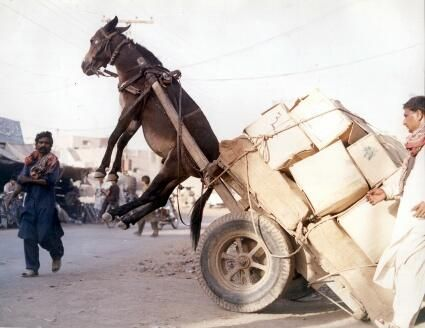
\includegraphics[scale=0.45]{img/ia.jpg}
    \end{center}
\end{frame}

\begin{frame}{Когда это бывает?}
    \begin{block}{Достигнуты технические ограничения}
        \begin{itemize}
            \item Сеть
            \item Память
            \item CPU
            \item Хранилище
        \end{itemize}
    \end{block}
    \begin{block}{Дополнительно}
        \begin{itemize}
            \item Недоиспользование железа
            \item Трудности масштабирования
        \end{itemize}
    \end{block}
\end{frame}

\begin{frame}{Причина}
    \begin{block}
        {\huge Архитектурные проблемы}
    \end{block}
\end{frame}

\begin{frame}{Недоиспользование железа}
    Рассмотрим типичный вебсервер на Perl, Python, Ruby...
    \pause

    \begin{columns}
        \column{.5\textwidth}
        \begin{block}{Задачи одного цикла}
            \begin{itemize}
                \item Чтение запроса из сети.
                \item Парсинг запроса http.
                \item Валидация запроса, выбор контроллера.
                \item Запрос(ы) к хранилищу данных.
                \item Формирование ответа (template).
                \item Отправка ответа клиенту.
            \end{itemize}
        \end{block}

        \pause
        \column{.5\textwidth}
        \begin{block}{Традиционная реализация (apache)}
            \begin{itemize}
                \item один процесс на один цикл
                \item один тред на один цикл
            \end{itemize}

        \end{block}
    \end{columns}
\end{frame}


\begin{frame}{Недоиспользование железа}
    \begin{block}{Начались разговоры о HighLoad?}
        \begin{itemize}
            \item Увеличение числа процессов/тредов.
            \item Увеличение числа серверов.
        \end{itemize}
    \end{block}
\end{frame}

\begin{frame}{Недоиспользование железа}
    \begin{block}{Вернемся к рассматриваемому серверу}
        \begin{itemize}
            \item Проблемы наступили при $\approx$100 запросах в секунду.

            \item Увеличили число процессов в работе.
                \par - Помогло.

            \item Новые проблемы при $\approx$150 запросов в секунду.

            \item Дальнейшее увеличение числа процессов помогает слабо.
        \end{itemize}
    \end{block}
\end{frame}

\begin{frame}{Недоиспользование железа}
    \begin{columns}
        \column{.5\textwidth}
        \begin{block}{Что делать?}
            \begin{itemize}
                \pause\item Переписывать?
                    \pause\par - Мы над этим 3 года работали!

                \pause\item Добавлять второй сервер?
                    \pause\par - Это тоже не просто! (бизнеслогика)
            \end{itemize}
        \end{block}

        \column{.5\textwidth}
        \begin{block}{Спокойно!}
            \begin{itemize}
                \item Провести измерения.
                \item Провести анализ архитектуры.
                \item Найти слабые места.
            \end{itemize}
        \end{block}
    \end{columns}
\end{frame}

\begin{frame}{Недоиспользование железа}
    \begin{block}{Измерения}
        \begin{tabular}{ c c }
            Чтение запроса из сети. & 15К RPS  \\
            Парсинг запроса, контроллер. & 150К RPS/CPU  \\
            Запросы к хранилищу. & 60К RPS \\
            Формирование ответа & 100К RPS/CPU \\
            Отправка ответа клиенту. & 15К RPS \\
        \end{tabular}
    \end{block}
\end{frame}


\begin{frame}{Недоиспользование железа}
    \begin{block}{Итого}
        {\huge
            $\frac{1}{                                      %
                \frac{1}{15 \cdot 10^3} +                   %
                \frac{1}{150 \cdot 10^3} +                  %
                \frac{1}{60 \cdot 10^3} +                   %
                \frac{1}{100 \cdot 10^3} +                  %
                \frac{1}{15 \cdot 10^3}} = 6000 RPS$
        }
    \end{block}

    \pause
    \begin{block}{Но, позвольте!}
        \begin{itemize}
            \item У нас проблемы на 150 RPS!
            \item Тут что-то не так!
        \end{itemize}
    \end{block}
\end{frame}


\begin{frame}{Недоиспользование железа}
    \begin{block}{Начинаем разбираться}
        \begin{itemize}
            \item Хранилище выходит на свои RPS при достаточно большом
                числе соединений к нему.
            \item Либо хранилище надо располагать локально.
                \par {\small неприемлемо.}
            \item То же самое и с взаимодействием с клиентом.
        \end{itemize}
    \end{block}
\end{frame}

\begin{frame}{Недоиспользование железа}
    \begin{block}{Резюме ситуации, еще раз}
        \begin{itemize}
            \item Имеется 100500 строк кода,
                над которым работали несколько лет.

            \item Этот код AS IS по результатам измерений
                может выдавать гораздо больше RPS чем в реальности.

            \item Проблемы начинаются на уровне RPS на порядок меньших,
                нежели расчетные.
        \end{itemize}
    \end{block}
\end{frame}


\begin{frame}{Недоиспользование железа}
    \begin{columns}
        \column{.5\textwidth}
            \begin{block}{Работа сервера}
                \begin{itemize}
                    \item Запросу выделяется CPU.
                    \item Ожидаются данные запроса.
                    \item Диспетчеризация.
                    \item Запросы в БД.
                    \item Ожидаются ответы из БД.
                    \item Формируется ответ.
                    \item Ответ отправляется клиенту.
                \end{itemize}
            \end{block}
        \pause
        \column{.5\textwidth}
            \begin{block}{Магазин обуви}
                \begin{itemize}
                    \item Клиенту выделяется менеджер.
                    \item Сопровождает клиента.
                    \item Может сходить на склад за нужным размером.
                    \item Ожидает товара со склада/решения клиента.
                    \item Пробивает чек на кассе.
                    \item Прощается с клиентом.
                \end{itemize}
            \end{block}
    \end{columns}
\end{frame}


\begin{frame}{Недоиспользование железа}
    \begin{block}{Измеряем}
        \begin{tabular}{ c c }
            Ожидание запроса (данных) от пользователя. & 70 мкс \\
            Парсинг запроса, валидация.  & 6 мкс \\
            Формирование запроса (запросов) в БД. & 1 мкс \\
            Ожидание ответа (ответов) из БД. & 16 мкс \\
            Соединение данных из БД с шаблоном. & 10 мкс\\
            Ожидание отправки данных клиенту. & 70 мкс \\
        \end{tabular}
    \end{block}
\end{frame}

\begin{frame}{Недоиспользование железа}
    \begin{block}{Итого}
        \begin{itemize}
            \item Код выполнялся: $6 + 1 + 10 = 17$ мкс
            \item Чего-либо ожидали: $70 + 16 + 70 = 156$ мкс
            \pause\item {\large Код выполняется только 10\% времени!}
            \item И при этом тормозит!
        \end{itemize}
    \end{block}
\end{frame}

\begin{frame}[fragile]{Недоиспользование железа}
\begin{verbatim}
#include <unistd.h>

int main(int argc, char **argv) {
        int i;
        for (;;) {
                usleep(70);     usleep(7);
                usleep(17);     usleep(10);
                usleep(70);
        }
}
\end{verbatim}
\end{frame}

\begin{frame}{Недоиспользование железа}
    \begin{block}{Итого}
        \begin{itemize}
            \item Код, делающий только sleep в цикле неплохо грузит CPU
                \par - по моим измерениям - где-то 15\% загрузки на CPU
            \item Запустив десяток таких ``воркеров'', получаем
                примерно такую же нагрузку как на проблемном сервере.
            \item Понятно что пример синтетический
                (есть вопросы к реализации usleep).
        \end{itemize}
    \end{block}

    \pause
    \begin{block}{Вернемся к нашему серверу}
        \begin{itemize}
            \item Каждая отдельная часть имеет хорошую производительность
                \par достаточную для развития
                            проекта еще на несколько лет вперед.
            \item Большую часть времени (90\%) наш код проводит
                        в ожидании.

            \item Что делать?
        \end{itemize}
    \end{block}
\end{frame}

\begin{frame}{Недоиспользование железа}
    \begin{block}
        {\huge Просто реорганизовать код}
            \begin{center}
                \pause
\includegraphics[scale=0.35]{img/nelzya.png}
            \end{center}
    \end{block}
\end{frame}


\begin{frame}{Событийно-ориентированное программирование}

    \begin{quote}
    Компьютер — это конечный автомат.
        Треды для тех людей, которые не умеют
        программировать конечные автоматы.
    \end{quote}
    \begin{center}
        \begin{uncoverenv}
        Алан Кокс
        \end{uncoverenv}
    \end{center}

\end{frame}

\begin{frame}{Событийно-ориентированное программирование}
    \begin{block}
        {\huge Избавимся от тредов!}
            \par - {\small и процессов.}
    \end{block}
\end{frame}


\begin{frame}{От магазина обуви к продуктовому!}
    \begin{block}{Особенности продуктового магазина}
        \begin{itemize}
            \item Клиенты собираются в очереди.
            \item Продавец обслуживает клиентов по очереди и без простоя.
            \item Простой продавца возможен только при отсутствии клиентов.
            \item Один продавец может обслужить в десятки раз больше клиентов.
            \item PROFIT?
        \end{itemize}
    \end{block}

\end{frame}

\begin{frame}{Событийно-ориентированное программирование}
    \begin{block}{Машина событий}
        \begin{itemize}

            \item Исполнитель заявляет о готовности выполнить задачу.
                \par - подписывается на событие: ``Свободная касса!''

            \item При появлении задачи исполнитель начинает
                ее выполнение немедленно.

            \item Если задача требует ожидания - ставит ожидающего
                в очередь и переходит к выполнению другой задачи.

        \end{itemize}
    \end{block}

    \pause
    \begin{block}{Типичная реализация}
        \begin{itemize}
            \item Подписка на задачу - регистрация callback.
            \item Выполнение задачи - вызов callback.
            \item Ожидание - return из callback.
        \end{itemize}

    \end{block}
\end{frame}

\begin{frame}{Событийно-ориентированное программирование}
    \begin{block}{Перестроим наш сервер}
        \begin{itemize}
            \item Ожидание запроса от пользователя.
                \par - заменится регистрацией callback
                    "пришел запрос от пользователя"
            \item Диспетчерезация запроса - не изменится
            \item Формирование запросов в БД - не изменится
            \item Ожидание ответа из БД.
                \par - заменится регистрацией callback
                        "пришел ответ из БД"
            \item Формирование ответа - не изменится
            \item Ожидание отправки данных клиенту.
                \par - заменится регистрацией callback
                        "данные пользователю отправлены"
        \end{itemize}
    \end{block}
\end{frame}


\begin{frame}{Событийно-ориентированное программирование}
    \begin{block}{Переписываем одну страничку и изменяем}
        \begin{itemize}
            \item Производительность одного сервера выросла в >10 раз
            \item Одного CPU/коннекта к БД достаточно для еще нескольких
                лет роста нагрузки.

            \item Но слишком много переделок!
        \end{itemize}
    \end{block}

    \pause
    \begin{block}{Проблемы}
        \begin{itemize}
            \item Сохранение контекста между callback
            \item Ветвления
            \item Обработка исключительных ситуаций
        \end{itemize}
    \end{block}
\end{frame}


\begin{frame}{Событийно-ориентированное программирование}
    \begin{block}{Что затронуто изменениями}
        \begin{itemize}
            \item Интерфейс с вебсервером - некритично.
            \item Интерфейс с БД.
                \par - критично.
                Много кода бизнеслогики поехало в callbacks. Сложную логику
                практически невозможно реализовать.
                Требуется переписывание ~90\% проекта.
            \item Интерфейс с сетью (если он есть)
                \par - так же переехал в callbacks.
        \end{itemize}
    \end{block}
\end{frame}

\begin{frame}{Событийно-ориентированное программирование}
    \begin{block}{Плюсы Обувного магазина}
        \begin{itemize}
            \item Контекст задачи можно хранить на текущем стеке
                (свалить на менеджера).
            \item Процесс можно прервать в любой момент.
            \item Произвольное ветвление (можно ходить по разным
                отделам в произвольном порядке).
        \end{itemize}
    \end{block}

    \begin{block}{Плюсы продуктового магазина}
        \begin{itemize}
            \item Менеджеры не простаивают
        \end{itemize}
    \end{block}
\end{frame}

\begin{frame}{Событийно-ориентированное программирование}
    \begin{block}{Соединим плюсы обоих подходов}
        Пишем свой планировщик (fibers).
        \begin{itemize}
            \item Невытесняющая многозадачность
            \item Простое порождение ``процессов''
            \item Простое API
                \par Три основных метода
                \begin{itemize}
                    \item Создать процесс (create, async)
                    \item Передать управление планировщику (yield, cede)
                    \item Разбудить выбранный процесс (wakeup, ready)
                \end{itemize}
        \end{itemize}
    \end{block}
\end{frame}

\begin{frame}{Событийно-ориентированное программирование}
    \begin{block}{Интеграция планировщика с машиной событий}
        Структура кода теперь выглядит так:
        \begin{itemize}
            \item Подписка на событие (регистрация callback).
            \item Передача управления планировщику (yield, cede).
            \item Событие будит (wakeup) текущий процесс.
            \item Процесс обрабатывает события используя данные переданные
                в callback.
        \end{itemize}
    \end{block}
    \pause
    \begin{block}{Итого}
        Вернулись к (почти) традиционному виду программы.
    \end{block}
\end{frame}

\begin{frame}{Событийно-ориентированное программирование}
    \begin{block}{Вернемся к нашему серверу}
        \begin{itemize}
            \item Добавляем машину событий
            \item Добавляем библиотеку fibers
            \item Переписываем интерфейс с вебсервером (врапперы).
            \item Переписываем интерфейс с БД (врапперы).
            \item Переписываем другие сетевые обращения (если есть).

            \pause\item Итого: переписываем около 5\% кода.
            \item PROFIT!
        \end{itemize}
    \end{block}
\end{frame}

\begin{frame}{Библиотеки и языки}
    \begin{itemize}
        \pause\item Perl
            \pause\par Coro + AnyEvent
        \pause\item Python
            \pause\par fibers + twisted
        \pause\item PHP5
            \pause\par появился оператор yield, fiber
    \end{itemize}
\end{frame}

\begin{frame}{Что дальше?}
    \begin{itemize}
        \item Используем fiber'ы/event-машины
            в том языке к которому привыкли
        \item Рассматриваем существующие варианты
            \begin{itemize}
                \item Node.JS
                    \par - отказались от парадигмы fibers
                    \par но в последнее время появились подвижки.
                \item\pause Tarantool...
            \end{itemize}
    \end{itemize}
\end{frame}


\begin{frame}{Tarantool}
    \begin{itemize}
        \item Полноценный app-сервер
        \item fibers, libev
        \item БД на борту
            \par - in-memory
            \par - disk
        \item Сокеты, диск, http-сервер, очереди
    \end{itemize}
\end{frame}

\begin{frame}{Недостатки подхода}
    \begin{itemize}
        \item Для больших проектов одного CPU все-таки маловато
        \item Реализации fiber'ов для традиционных
            ЯП плохо масштабируются по CPU/хостам.
    \end{itemize}
\end{frame}

\begin{frame}{Перспектива}
    \begin{itemize}
        \item Erlang
            \par - хорошее масштабирование по CPU и хостам
            \par - очень качественное решение
            \par - высокий порог вхождения
        \item Go
            \par - более низкий порог вхождения
    \end{itemize}
\end{frame}

\begin{frame}{Наутакси}
    Крупнейший бакенд Яндекс.Такси.
    \begin{itemize}
        \item 20.000+ водителей непрерывно шлют свое местоположение
        \item > 1 млн заявок на заказы в мес
        \par\pause
    \end{itemize}

    Проект включает в себя:
    \begin{itemize}
        \item Вебсервер на Coro+AnyEvent
        \item Большую коллекцию очередей на Tarantool
        \item Систему доставки сообщений на Tarantool
        \item Хранилище данных на PostgreSQL
    \end{itemize}
\end{frame}

\begin{frame}{Наутакси}
    \begin{columns}
        \column{.5\textwidth}
            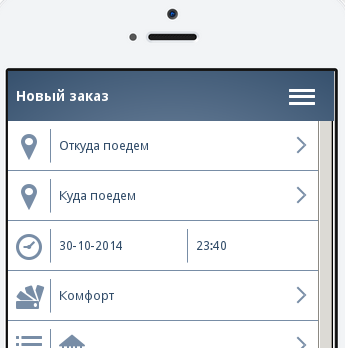
\includegraphics[scale=0.8]{img/nowtaxi.png}
        \column{.5\textwidth}
        
        Проект обслуживает:
        \begin{itemize}
            \item Мобильное приложение клиента
            \item Мобильные приложения водителя
            \item Систему управления диспетчерскими
            \item Мониторинг
            \par
            \item Все помещается на двух хостах на Hetzner
        \end{itemize}
    \end{columns}
\end{frame}

\begin{frame}{Наутакси}
    \begin{block}{Фичи}
        \begin{itemize}
            \item Можно заказать такси (подача от 5 минут)
            \item и эвакуатор
        \end{itemize}
    \end{block}

    \begin{block}{Ссылки}
        \begin{itemize}
            \item AppleStore://Наутакси
            \item PlayMarket://Наутакси
        \end{itemize}
    \end{block}

\end{frame}

\begin{frame}
    \begin{center}
        {\huge Дзен}
    \end{center}
\end{frame}


\begin{frame}{HighLoad и базы данных}
    \begin{block}{Что делать?}
        \begin{itemize}
            \item Переезжать на другое железо?
            \item Переходить на другую БД?
        \end{itemize}
        \par
        \begin{itemize}
            \pause\item Опять смотреть на архитектуру!
        \end{itemize}
    \end{block}
\end{frame}


\begin{frame}{Вопрос}
    \begin{center}
        {\huge Что представляет из себя любая БД?}
    \end{center}
\end{frame}

\begin{frame}{Философия: что такое БД?}
    \begin{itemize}
        \pause\item Массив записей.
    \end{itemize}
\end{frame}

\begin{frame}{Философия: что такое БД?}
    \begin{itemize}
        \item Несколько массивов записей.
        \pause\item Средства ускорения поиска по массиву (индексы).
        \pause\item И...\pause ВСЕ!
    \end{itemize}
\end{frame}

\begin{frame}{Виды поисков по массиву}
    \begin{itemize}
        \item Сканирование: $O(N)$
        \item Индексированный: $O(\ln N)$ (иногда $O(1)$).
    \end{itemize}
\end{frame}

\begin{frame}[fragile]{Выбор из двух массивов: JOIN}
\begin{verbatim}
SELECT
    *
FROM
    "users"
JOIN
    "roles" ON "users"."id" = "roles"."uid"
WHERE
        "roles"."id" IN (10, 20, 30)
    AND "users"."id" IN (30, 40, 50)
\end{verbatim}
\end{frame}

\begin{frame}{Выбор из двух массивов: JOIN}
    \begin{itemize}
        \item Выбираются записи первого массива $K1 \cdot O(\ln{N1})$
            \par {\small $K1$ определяется на стадии
                выборки из первого индекса}
        \item Сопоставляются записям второго: $K2 \cdot O(\ln{N2})$
            \par {\small На этом шаге становится известным $K2$}
        \item Результат фильтруется: $O(K2)$ по условиям,
          если таковые еще не отфильтрованы.
    \end{itemize}

    \begin{block}{Итого}
        $K1 \cdot O(\ln{N1}) + K2 \cdot O(\ln{N2}) + O(K2)$
    \end{block}
\end{frame}

\begin{frame}{Пути оптимизации?}
    \begin{itemize}
        \item Попытаться предсказать что меньше $K1$ или $K2$
        \item Последовательные элементы из индекса иногда
            можно выбрать за время $\ln{N} + K1 \cdot c$
        \item Фильтрация на стадии JOIN

        \item И... все?!

        \pause\item Денормализация.
    \end{itemize}
\end{frame}

\begin{frame}{Усложняем задачу}
    \begin{itemize}
        \item Увеличиваем число таблиц в JOIN
        \item Вводим дополнительные условия WHERE
        \item Даже оценить ресурсы на выполнение запросов
            становится сложно.
    \end{itemize}
\end{frame}

\begin{frame}{Поговорим об интересном}
    \begin{block}
        {\huge Почему популярны NoSQL?}
        \begin{center}
            \pause
\includegraphics[scale=0.2]{img/Trollface_HD.png}
        \end{center}
    \end{block}
\end{frame}

\begin{frame}{Почему популярны NoSQL?}
    \begin{itemize}
        \pause\item Они более быстрые?
            \pause\par см. соседние доклады:
                PostgreSQL быстрее MongoDB в 10 раз.

        \pause\item Позволяют хранить слабоструктурированные данные?
            \pause\par hstore, arrays, composite появились в PostgreSQL
                много лет назад.

        \pause\item Шардинг/репликация?
            \pause\par решения для PostgreSQL существуют в избытке.

        \pause\item Может быть NoSQL имеют лучшие возможности
            по предсказанию плана выполнения запроса?
            \pause\par большинство NoSQL не умеет JOIN.

        \item Что еще?
    \end{itemize}
\end{frame}

\begin{frame}{Философия: что такое БД?}
    \begin{itemize}
        \item Массив(ы) записей.
        \item Индексы.
    \end{itemize}
\end{frame}

\begin{frame}{Почему популярны noSQL?}
    \begin{itemize}
        \pause\item Они не умеют JOIN.
        \pause\item Это заставляет программиста помнить о том что такое БД.
        \pause\item Положительно влияет на архитектуру приложения.
    \end{itemize}
\end{frame}

\begin{frame}{О БД Tarantool}
    \begin{itemize}
        \pause\item Это не БД.
        \pause\item Это APP-сервер с БД на борту.
        \pause\item JOIN не нужны: денормализация.
    \end{itemize}
    \begin{center}
        
\includegraphics[scale=0.2]{img/Trollface_HD.png}
    \end{center}
\end{frame}


\usebackgroundtemplate{%
    
\includegraphics[width=\paperwidth,height=\paperheight]{img/main-page.jpg}%
}

\begin{frame}
\end{frame}
\end {document}
